% !TEX root = thesis.tex
% =====================================================================
%  CHAPTER 1 — INTRODUCTION
%  Zero-Shot Nutrient and Quantity Association using
%  OCR-Guided Semantic Graph Matching
%  Moustafa Hamada | THD + USB
%
%  Build: scrbook, XeLaTeX + BibTeX. Citations: \cite{}.
%  Cross-refs: Chapter~\ref{} / Section~\ref{}  (matches the Ch2/Ch5/Ch6 body).
%
%  REVISION NOTES (this pass):
%    - Motivation no longer lists specific downstream applications; the value of
%      structured label data is stated generally.
%    - Motivation now names the large-VLM shortcut and its two costs (price and
%      the black-box lack of transparency), and this tension is carried through
%      the problem statement, the gap, and the research questions.
%    - A teaser figure reuses the Ch2 association-task image (Option A: same
%      asset, NEW label, teaser caption pointing to Ch2 — no other file touched).
%    - Aim section adds a central research question and a paragraph mapping the
%      five sub-questions to the dimensions of the research gap.
%
%  FORWARD REFERENCES (labels defined in the other chapter files):
%    chap:background   (Ch2)
%    ch:related-work   (Ch3 — note: this chapter keeps the ch: prefix, not chap:)
%    chap:methodology  (Ch4)
%    chap:evaluation   (Ch5)
%    chap:experiments  (Ch6)
%    chap:conclusion   (Ch7 — NOT YET WRITTEN. Use exactly this label in the
%                       conclusion file so the \ref here resolves; until then
%                       LaTeX prints "??" for that one reference only.)
%
%  FIGURE ASSET (reused from Ch2, guarded by \IfFileExists so it compiles before
%  the file is present):
%    association_task.png   ->  \label{fig:intro-association-task}
%
%  CITED KEYS — all already appear in references.bib (reused from Ch3/Ch4):
%    nagayi2025foodocr, arief2026halalbench, yu2020pick, hwang2021spade
%
%  NOTE: \mcode{} is defined *inside* Chapter 4, so it is NOT available here.
%  Any code-like literal in this chapter uses \texttt{} instead.
%
%  LABELS IN THIS FILE:
%    chap:introduction
%    sec:intro-motivation, sec:intro-problem, sec:intro-gap,
%    sec:intro-questions, sec:intro-contributions, sec:intro-outline
% =====================================================================

\chapter{Introduction}\label{chap:introduction}

Packaged food and dietary supplements carry a nutrition label, and for most
products that printed panel is the main public record of what the product
contains. Having its contents as structured data --- one clean record per
nutrient value --- is far more useful than the image itself, because structured
records can be searched, compared, and processed automatically, while an image
cannot. This thesis builds a system that reads the label image, works out which
number belongs to which nutrient, and returns the result as a set of such
records, without being trained on the labels it must read.

\section{Motivation}\label{sec:intro-motivation}

A nutrition or supplement label is a small, dense document. It lists the
product's nutrients, the amount of each, the unit that amount is measured in, and
the reference basis the amount is stated under, such as per 100 grams or per
serving. Written as a record, one such line becomes the four-field tuple
$\langle\text{nutrient},\,\text{quantity},\,\text{unit},\,\text{context}\rangle$.
A person can read a panel one line at a time, but many uses need the data for many
products at once, in a form a program can process, and producing that by hand
does not scale: the set of products is open and grows constantly, with tens of
thousands of new layouts appearing each year, each of which would have to be
transcribed and checked. An automatic method that reads the label image and
returns the records directly is therefore worth having.

One modern shortcut is to hand the whole task to a large vision--language model:
give it the label image and ask it to return the records in a single step. Such a
model needs no task-specific training and copes with many layouts, which makes it
an obvious first choice. It comes with two costs, though, that matter for this
setting. The first is price: calling a large model on every label is expensive,
and the expense grows with the number of labels. The second, and the more serious
here, is that the model is a black box. It returns the records in one opaque step,
with no intermediate that can be inspected, so when a value comes out wrong there
is no way to tell whether the mistake was in the reading, the classification, or
the linking, and no record tying an output back to the evidence that produced it.
For data meant to be processed automatically, being unable to check or trace a
result is a real limitation. What is wanted, then, is a method that is automatic
like the model, but also cheap to run and open to inspection at every step. That
is the method this thesis sets out to build.

\section{Problem Statement}\label{sec:intro-problem}

The first step, optical character recognition (OCR), reads the characters in the
image and returns them as text tokens, each with a bounding box and a confidence
score. This is necessary but not sufficient. OCR says what text is on the label
and where it sits; it does not say how the pieces belong together. A label carries
many nutrient names and many numbers, and the real work is to join each number to
the nutrient it describes, then attach the right unit and the right context. This
joining step is the association problem, and it is the heart of the task. Seeing
the tokens \texttt{Magnesium}, \texttt{400}, and \texttt{mg} on a label is not the
same as knowing that the three form one record; a label may hold twenty nutrients
and forty numbers, and a single wrong link already produces a wrong record.
Figure~\ref{fig:intro-association-task} shows the task end to end: the label
enters on the left, its classified tokens sit in the middle, and the finished
records leave on the right, with the association step marked by the question mark.

\begin{figure}[htbp]
  \centering
  \IfFileExists{association_task.png}{%
    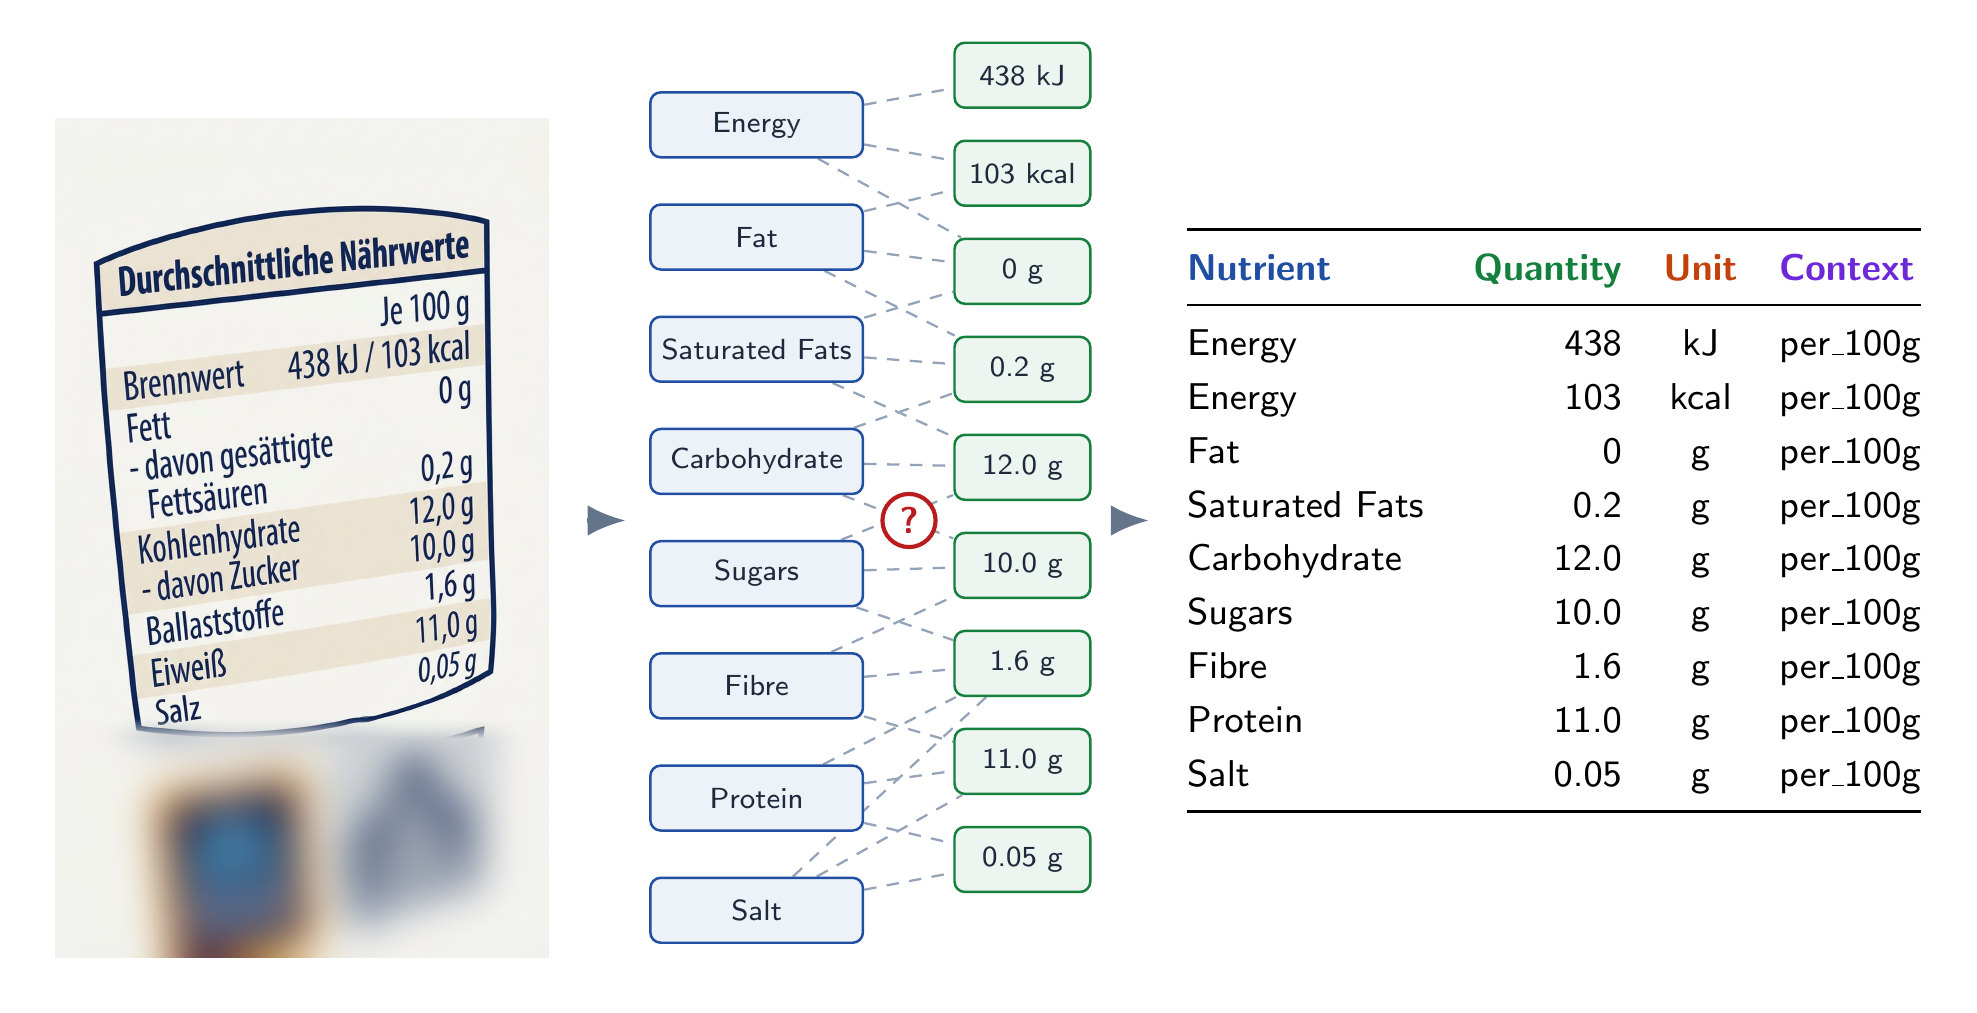
\includegraphics[width=\textwidth]{association_task.png}%
  }{%
    \fbox{\parbox[c][0.30\textheight][c]{0.9\textwidth}{\centering\itshape
      Figure file \texttt{association\_task.png} not found --- save the
      association-task figure to this path.}}%
  }
  \caption[The extraction task at a glance]{The extraction task at a glance, on
    one nutrition label. \emph{Left:} the input image. \emph{Middle:} the same
    tokens after classification, with nutrient names on one side and quantities
    on the other. \emph{Right:} the target records, one four-field tuple per row.
    The association step, marked by the question mark, must tie each quantity to
    the correct nutrient; because a label holds many of each, one wrong link
    already yields a wrong record. The same figure, with the full definition,
    appears in Chapter~\ref{chap:background}.}
  \label{fig:intro-association-task}
\end{figure}

Several properties of real labels make association hard. The labels are
multilingual: a single panel often mixes German and English, and others across
the corpus add French, Dutch, Italian, and Spanish. They are laid out as dense
tables, sometimes photographed at an angle or printed on curved packaging, so the
geometry is not clean; both failure modes are well documented for food-packaging
OCR~\cite{nagayi2025foodocr}. Most of all, the labels are multi-context. The same
nutrient is frequently reported more than once --- once per 100 grams and once
per serving, for example --- so one nutrient name lines up with several numbers,
and the only thing that separates those numbers is the column each sits in.
Across the corpus used here, about two-thirds of nutrient instances carry more
than one value in this way. A method that reads the label line by line cannot tell
these values apart; it has to reason about the column layout, which is what makes
a simple left-to-right or top-to-bottom reading insufficient.

The task also has to be solved without training on the labels themselves. There
is no annotated corpus of supplement labels with record-level ground truth to
learn from, and building one for a fixed set of products would not help for long,
since the set of products is open and keeps growing. The wide spread of real
labels makes this concrete --- a large multilingual benchmark finds that even
strong engines fail on scripts they were not built for~\cite{arief2026halalbench}
--- so any method that depends on per-layout or per-language training cannot
scale. The system must therefore work zero-shot, on nutrient names, layouts, and
languages it has not met before, and lean on general-purpose components and
explicit rules rather than on a model fitted to the target labels. In this thesis
the constraint is taken strictly: no stage is trained or fine-tuned on the label
images, and the annotations are used only to score the output, never to build it.

The interpretability that the motivation calls for is the last requirement, and
the multi-stage design is what delivers it. Where an end-to-end model binds every
field in one opaque step, a pipeline that keeps its stages explicit --- each token
carrying its text, role, and position, and each link traceable to the rule that
made it --- can be inspected when a record is wrong and corrected at the stage
that caused it. This thesis therefore treats interpretability as a design goal on
equal footing with accuracy, and its components are chosen so that the reasoning
behind each record stays visible.

\section{Limitations of Existing Approaches}\label{sec:intro-gap}

Existing methods each solve part of this problem but give up something the task
needs. Chapter~\ref{ch:related-work} reviews them in full; only the shape of the
gap is given here. Pipelines built on OCR followed by regular expressions or
hand-written rules are transparent and need no training, but they break on the
structural problems above --- dense rows of numbers, several value columns, mixed
languages, and broken layouts. Graph-based extractors such as PICK~\cite{yu2020pick}
and SPADE~\cite{hwang2021spade} rightly treat extraction as a relational problem
and reason over the two-dimensional layout, but they learn their structure end to
end from annotated corpora, so they are not built for zero-shot use across unseen
multilingual labels, and no such annotated corpus of supplement labels exists to
train them on. End-to-end vision--language models, already discussed above, remove
the need for training data but return their records from a single step that is
costly to run and cannot be inspected, with no audit trail from an output back to
its evidence.

Read together, these approaches leave one corner of the design space empty. None
is at once zero-shot, interpretable, relational, and able to handle multilingual
labels: the regex pipelines are not robust, the graph extractors are not
zero-shot, and the end-to-end models are not interpretable. No existing method
reconstructs four-field nutrition tuples from arbitrary, multilingual, previously
unseen supplement labels without task-specific training while keeping every stage
open to inspection. That corner is what this thesis sets out to occupy.

\section{Aim and Research Questions}\label{sec:intro-questions}

The aim of this thesis is to build a modular, interpretable, zero-shot pipeline
that reconstructs the four-field tuple
$\langle\text{nutrient},\,\text{quantity},\,\text{unit},\,\text{context}\rangle$
from an arbitrary multilingual nutrition or supplement label. The approach keeps
OCR as a replaceable front-end that supplies tokens, classifies each token into a
semantic role without training on the target labels, and then solves the
association problem with an explicit graph. This graph is the central idea of the
work, named here OCR-guided semantic graph matching: the classified tokens become
nodes, and typed edges --- built by closed-form geometric and structural rules
rather than learned weights --- record which tokens are aligned in a row, share a
column, sit next to one another, or fall under the same header. The output records
are then read back out of the graph. Because the edges follow fixed rules, the
same label always gives the same edges, and every link can be traced to the rule
behind it, which keeps the association step interpretable while remaining
zero-shot.

A vision--language model is included, but deliberately confined. Rather than hand
the whole task to such a model, the pipeline uses one only at the association
step, giving it the same OCR-derived token table the graph receives and asking it
to bind the tokens into records. This variant is a point of comparison, not the
primary method, and it is set against a second use of the same class of model that
maps the raw image straight to records end to end. Comparing the graph, the
confined model, and the end-to-end model shows how much of the result comes from
structuring the problem before any field is bound, and how much comes from the
model's flexibility.

These aims come together in one central question:
\begin{quote}
Can a modular pipeline that stays zero-shot and interpretable at every stage
reconstruct the four-field tuple from arbitrary multilingual supplement labels by
matching a semantic graph over OCR tokens, and how does it compare, in both
accuracy and cost, with confining a vision--language model to the association step
and with an end-to-end vision--language model?
\end{quote}
The question restates the four properties the research gap leaves unmet ---
zero-shot, interpretable, graph-based, and multilingual --- and adds the
comparison against the black-box alternative that the motivation set up.

The pipeline is modular, so each part of this question can be tested on its own by
changing one stage while the rest is held fixed. The central question therefore
breaks into five sub-questions, each tied to one design choice and answered by
ablation in Chapter~\ref{chap:experiments}:
\begin{enumerate}
  \item Which OCR engine reads nutrition labels most accurately?
  \item Which semantic classifier detects nutrient entities most reliably?
  \item Which association engine builds better tuples, the naive geometric graph
        or the enriched, geometry-aware graph?
  \item If a vision--language model is used only at the association step, does it
        beat the graph, and how does it compare with an end-to-end
        vision--language model that maps the image directly to tuples?
  \item Which edge-creation mode builds the best row relations inside the enriched
        graph?
\end{enumerate}

Each sub-question probes one dimension of the gap. Questions~1 and~2 concern the
zero-shot reading and classification the whole pipeline stands on, so they test
whether the interpretable front-end can recover the tokens at all without
training. Questions~3 and~5 are the core of the contribution: they ask whether a
graph built from closed-form geometric rules can do the relational binding that
PICK and SPADE reach only with supervision, and whether its geometric edges are
the right mechanism for it --- the answer to those extractors' reliance on
annotated data. Question~4 makes the interpretability-and-cost trade-off
measurable, weighing the fully interpretable graph against the confined and
end-to-end uses of a black-box model --- the answer to the opacity and expense of
end-to-end extraction. Together the five cover the empty corner the gap describes,
from the reading substrate to the binding step.

\section{Contributions}\label{sec:intro-contributions}

The thesis makes the following contributions.
\begin{enumerate}
  \item A modular, fully interpretable, zero-shot extraction pipeline that
        reconstructs four-field nutrition tuples from multilingual supplement
        labels, with the intermediate output of every stage kept explicit so that
        a wrong record can be traced to the stage that caused it.

  \item Its central novelty, OCR-guided semantic graph matching: an association
        method that builds an explicit graph over semantically classified OCR
        tokens using closed-form geometric and structural edge rules, with no
        learned weights and no training on the target data. Its enriched,
        geometry-aware form keeps several value columns apart, which is where it
        earns its advantage on multi-context labels.

  \item A design that confines a vision--language model to the association
        sub-task alone, together with a controlled comparison of this confined
        model against the graph and against an end-to-end model, which isolates
        the value of structuring the problem before any field is bound and makes
        the cost of the black-box route explicit.

  \item An annotated evaluation corpus of 57 multilingual nutrition and supplement
        labels with 866 gold four-field tuples, together with a deterministic,
        fully reproducible evaluation protocol.

  \item A systematic ablation across three axes --- the OCR engine, the semantic
        classifier, and the association engine --- that separates the effect of
        each design choice on the final tuple score, and a set of empirical
        findings that follow from it: OCR is the single largest lever; the
        enriched graph's advantage over the naive one is structural and shows on
        multi-context labels; geometric row edges beat rank-based ones; confining
        a vision--language model to association beats using it end to end; and a
        clear trade-off holds between accuracy, interpretability, and runtime.
\end{enumerate}

\section{Thesis Outline}\label{sec:intro-outline}

The rest of the thesis is organised as follows.

Chapter~\ref{chap:background} fixes the vocabulary. It defines, in plain terms,
each idea the pipeline relies on --- structured extraction and association, OCR,
token normalisation, semantic role labelling, text embeddings, token enrichment,
graph representations, vision--language models, and zero-shot learning --- in the
order they appear in the pipeline.

Chapter~\ref{ch:related-work} sets these ideas against the published systems the
pipeline borrows from and departs from. It reviews OCR on food labels,
supervision-free information extraction, graph-based extraction, and zero-shot
extraction, and uses the comparison to state the research gap the thesis fills.

Chapter~\ref{chap:methodology} specifies the pipeline and the design decisions
behind it, stage by stage: OCR and token correction, semantic role
classification, token enrichment and geometry, graph construction, and
graph-based association, together with the confined vision--language association
variant. It also sets out the three ablation axes.

Chapter~\ref{chap:evaluation} describes the data and how the pipeline is scored.
It presents the 57-image corpus, the annotation schema and protocol, the four
scored fields, and the four-field and three-field tuple metrics with the matching
rules used for scoring.

Chapter~\ref{chap:experiments} presents the experiments and their results. It
answers the five questions above by ablation, changing one stage at a time across
the fourteen pipeline configurations, discusses what each comparison shows, and
analyses where the remaining errors begin.

Chapter~\ref{chap:conclusion} draws the findings together, states the limitations
of the method, and points to future work.